\section{Problem 2}
\textit{Using the CST microwave studio given at the course, design a Yagi-Uda antenna that has a gain of at least 6 dBi at 850 Mhz using the General Frequency (FEM) and IE solver. Compare the results and simulation time with the results from Matlab code and method of moments code form Agilent.}\\

We are using the same antenna design as described in \secref{sec:CST_implimented_Yagi}. Here we are only simulating in the frequency domain. 

\subsection{General Frequency (FEM) simulation}
The designed Yagi antenna in CST is giving a gain patten as shown in \figref{fig:yagi_3D_pattern_CSTfreq} when simulating in the frequency domain with FEM. The polar plot is shown in \figref{fig:yagi_pol_pattern_CSTfreq} we can see that the three elements Yagi-Uda antenna presents a gain of 8.9dBi. In \figref{fig:yagi_cart_pattern_CSTfreq} the Cartesian version is also presented.

\begin{figure}[!h]
  \centering
  \includegraphics[width=11cm]{yagi_3D_pattern_CSTfreq.eps}
  \caption{Figure showing the 3D gain patten of the CST designed antenna using FEM.}
  \label{fig:yagi_3D_pattern_CSTfreq}
\end{figure}

\begin{figure}[!h]
  \centering
  \includegraphics[width=11cm]{yagi_pol_pattern_CSTfreq.eps}
  \caption{Figure showing the polar gain patten of the CST designed antenna using FEM.}
  \label{fig:yagi_pol_pattern_CSTfreq}
\end{figure}

\begin{figure}[!h]
  \centering
  \includegraphics[width=11cm]{yagi_cart_pattern_CSTfreq.eps}
  \caption{Figure showing the Cartesian gain patten for the CST designed antenna using FEM.}
  \label{fig:yagi_cart_pattern_CSTfreq}
\end{figure}

\subsection{Integral Equation (IE) simulation}
The designed Yagi antenna in CST is giving a gain patten as shown in \figref{fig:yagi_3D_pattern_CSTie} when simulating in the frequency domain with IE. The polar plot is shown in \figref{fig:yagi_pol_pattern_CSTie} we can see that the three elements Yagi-Uda antenna presents a gain of 8.9dBi. In \figref{fig:yagi_cart_pattern_CSTie} the Cartesian version is also presented.

\begin{figure}[!h]
  \centering
  \includegraphics[width=11cm]{yagi_3D_pattern_CSTie.eps}
  \caption{Figure showing the 3D gain patten of the CST designed antenna using IE.}
  \label{fig:yagi_3D_pattern_CSTie}
\end{figure}

\begin{figure}[!h]
  \centering
  \includegraphics[width=11cm]{yagi_pol_pattern_CSTie.eps}
  \caption{Figure showing the polar gain patten of the CST designed antenna using IE.}
  \label{fig:yagi_pol_pattern_CSTie}
\end{figure}

\begin{figure}[!h]
  \centering
  \includegraphics[width=11cm]{yagi_cart_pattern_CSTie.eps}
  \caption{Figure showing the Cartesian gain patten for the CST designed antenna using IE.}
  \label{fig:yagi_cart_pattern_CSTie}
\end{figure}